%%%%%%%%%%%%%%%%%%%%%%%%%%%%%%%%%%%%%%%%%%%%%%%%%%%%
%% Here are the helpfull stuff
%%%%%%%%%%%%%%%%%%%%%%%%%%%%%%%%%%%%%%%%%%%%%%%%%%%%
\chapter{Combinational Logic Building Blocks}
\graphicspath{ {./chapter04/FigWork} }

\subsection{Helpful Stuff}
The following is a list of the devices covered in this chapter.

\begin{tabular}{|l|p{3.5in}|} \hline
    Nomenclature:  & N:M decoder                \\ \hline
    Data Input:    & 1-bit D        \\ \hline
    Data Output:   & M-bit vector $y = y_{M-1} \ldots y_1 y_0$    \\ \hline
    Control:       & N-bit vector $s = s_{N-1} \ldots s_1 s_0$    \\ \hline
    Status:        & none                    \\ \hline
    Behavior:      & $y_s = D$ all other outputs equal 0    \\ \hline
\end{tabular}

\begin{tabular}{|l|p{3.5in}|} \hline
    Nomenclature:  & N:1 multiplexer                        \\ \hline
    Data Input:    & M-bit vector $y=y_{M-1} \ldots y_1 y_0$    \\ \hline
    Data Output:   & 1-bit F          \\ \hline
    Control:       & $log_2(N)$-bit vector $s = s_{log_2(N)} \ldots s_1 s_0$    \\ \hline
    Status:        & none                                   \\ \hline
    Behavior:      & $F = y_s$                \\ \hline
\end{tabular}

\begin{tabular}{|l|p{3.5in}|} \hline
    Nomenclature:  & N-bit adder subtractor                 \\ \hline
    Data Input:    & two N-bit vectors $A$ and $B$           \\ \hline
    Data Output:   & N-bit vector  $s$               \\ \hline
    Control:       & 1-bit $c$                     \\ \hline
    Status:        & 1-bit ovf                 \\ \hline
    Behavior:      & if c=0 then $s = A+B$ else $s=A-B$     \\ \hline
\end{tabular}

\begin{tabular}{|l|p{3.5in}|} \hline
    Nomenclature:  & N-bit comparator                \\ \hline
    Data Input:    & two N-bit vectors $X$ and $Y$           \\ \hline
    Data Output:   & none               \\ \hline
    Control:       & none                      \\ \hline
    Status:        & 1-bit $G,L,E$ \\ \hline
    Behavior:      &
    $$
    \begin{array}{l|l|l|l}
        cond  & E & L & G \\ \hline
        X = Y & 1 & 0 & 0 \\ \hline
        X < Y & 0 & 1 & 0 \\ \hline
        X > Y & 0 & 0 & 1 \\
    \end{array}$$            \\ \hline
\end{tabular}

%%%%%%%%%%%%%%%%%%%%%%%%%%%%%%%%%%%%%%%%%%%%%%%%%%%%
%% Here are terms that the students define
%%%%%%%%%%%%%%%%%%%%%%%%%%%%%%%%%%%%%%%%%%%%%%%%%%%%
\subsection{Definitions}
\begin{description}
    \item [Data in]
    \item [Control]
    \item [Data out]
    \item [Status]
\end{description}

%%%%%%%%%%%%%%%%%%%%%%%%%%%%%%%%%%%%%%%%%%%%%%%%%%%%
%% Here are the problems
%%%%%%%%%%%%%%%%%%%%%%%%%%%%%%%%%%%%%%%%%%%%%%%%%%%%
\subsection{Problems}
Here are a couple of problems to work on.

\textbf{ Label the outputs of the decoder.}

\scalebox{0.5}{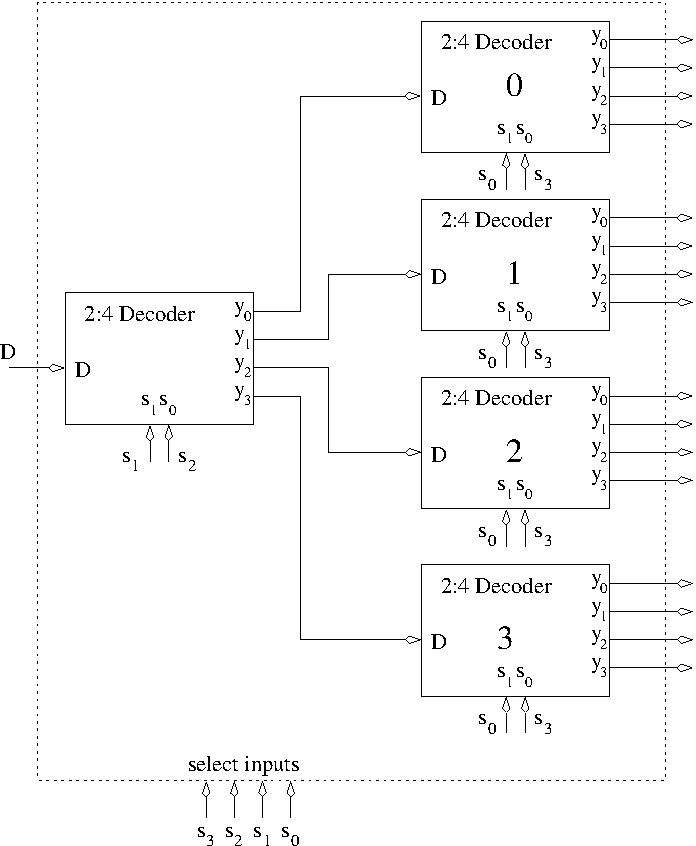
\includegraphics{OddDecoder}}

\textbf{ Label the inputs of the mux.}

\scalebox{0.5}{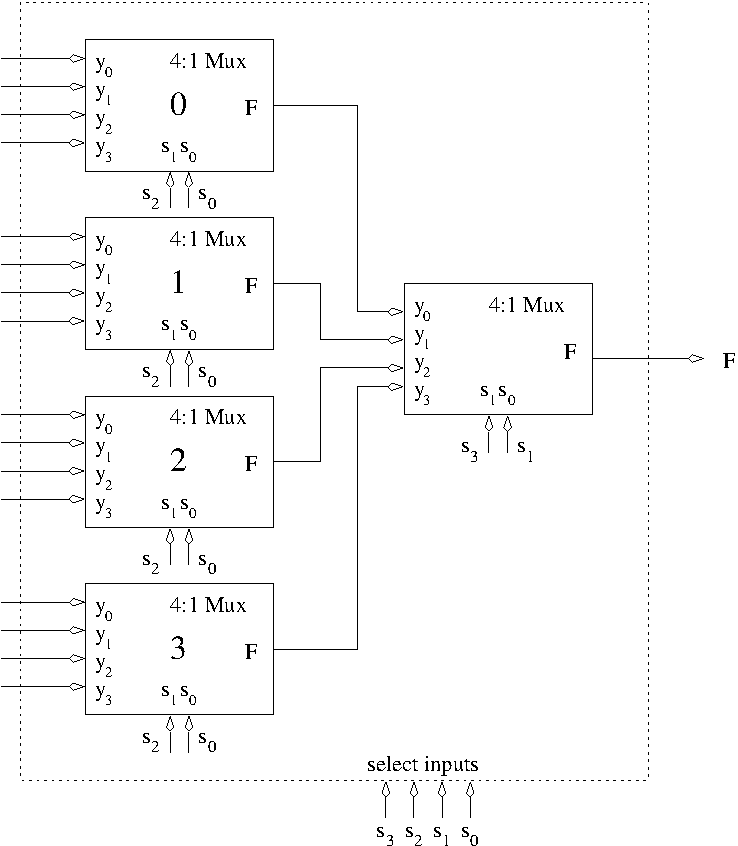
\includegraphics{OddMux}}

%% \item[Label all lines with their respective values.]
%% 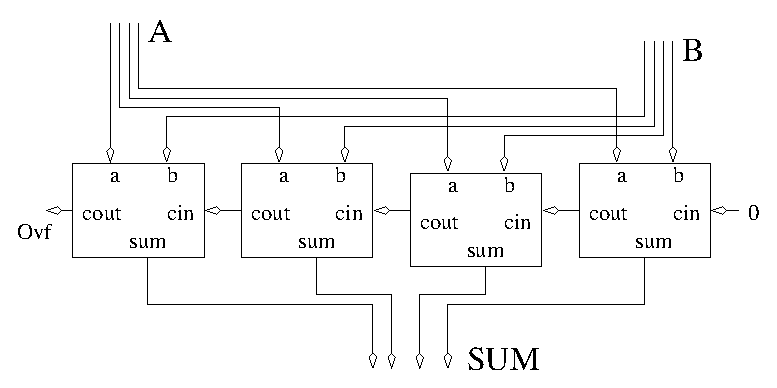
\includegraphics{./FigWork/adder}

\begin{description}

    \item[Build the circuit.]
\begin{verbatim}
if (Y<4) then X=2 else X=3
\end{verbatim}
        \vspace{1in}

    \item[Build the circuit.]
\begin{verbatim}
if (Y>=4) then X=Y+2 else X=Y+3
\end{verbatim}
        \vspace{1in}

    \item[Build the circuit.]
\begin{verbatim}
if (Y+1>15) then X=2 else X=3
\end{verbatim}

\end{description}
